% fyp_latex_includes.tex
% FYP Dissertation — LaTeX include snippets for all figures and tables.
% Generated by /paper-figure  |  2026-04-02  (data filled from hy-gpu server)
%
% Figure mapping (FYP numbering):
%   Fig. 1   = Hero / project arc           [MANUAL — ai_generated/fig1_hero_pipeline.png]
%   Fig. 2   = BER vs SNR traditional       [fyp_fig2_traditional_ber.pdf — real data: SNR=[15,20,25] dB]
%   Fig. 2b  = BER vs SNR corrector         [fyp_fig2b_corrector_ber_snr.pdf — real data: SNR=[5..25] dB]
%   Fig. 3   = Regime BER gains (forest)    [fyp_fig3_regime_gains.pdf] ✓
%   Fig. 4   = Feature ablation             [fig4_feature_ablation.pdf] ✓
%   Fig. 5   = Packet utility               [fig3_system_impact.pdf] ✓
%   Fig. 6   = Correction behavior          [fyp_fig6_correction_behavior.pdf] ✓ real data both panels
%   Table 1  = Traditional receivers        [TABLE1_traditional.tex — real BER at SNR=15 dB]
%   Table 2  = Method comparison (FYP)      [TABLE2_fyp_method_comparison.tex] ✓
%   Table 3  = Scope/claim matrix (FYP)     [TABLE3_fyp_claim_scope.tex] ✓
%   Table 4  = Complexity/overhead (FYP)    [TABLE4_fyp_complexity.tex — real values: 961 params]
%
% All items now have real data. No PLACEHOLDERs remain.
% Items marked [MANUAL] require manual creation (draw.io / TikZ).

% ─── Fig. 1: Hero / Project Arc ─────────────────────────────────────────────
% MANUAL — create in draw.io / Figma / TikZ.
% Existing AI-generated draft: figures/ai_generated/fig1_hero_pipeline.png
%
\begin{figure*}[t]
    \centering
    \includegraphics[width=0.96\textwidth]{figures/ai_generated/fig1_hero_pipeline.png}
    \caption{Project arc. The frozen direct-bit corrector (bottom path) is post-hoc, train-once,
             and scope-bounded. The mean-residual correction path (top) proved BER-neutral after
             evaluation protocol correction. The corrector targets sparse decision-boundary errors
             identified by oracle analysis, transfers positively across three regime shifts, and
             has an explicit failure boundary at $P_\text{paths}=15$.}
    \label{fig:hero_arc}
\end{figure*}

% ─── Fig. 2: BER vs SNR — Traditional Baseline Comparison ───────────────────
% Data: SNR=[15,20,25] dB, 100 frames each, seed=42.
% JointOMP-MP, TRADPARAM Fixed, TRADPARAM Classical Full, Stage6 Param Joint.
%
\begin{figure}[t]
    \centering
    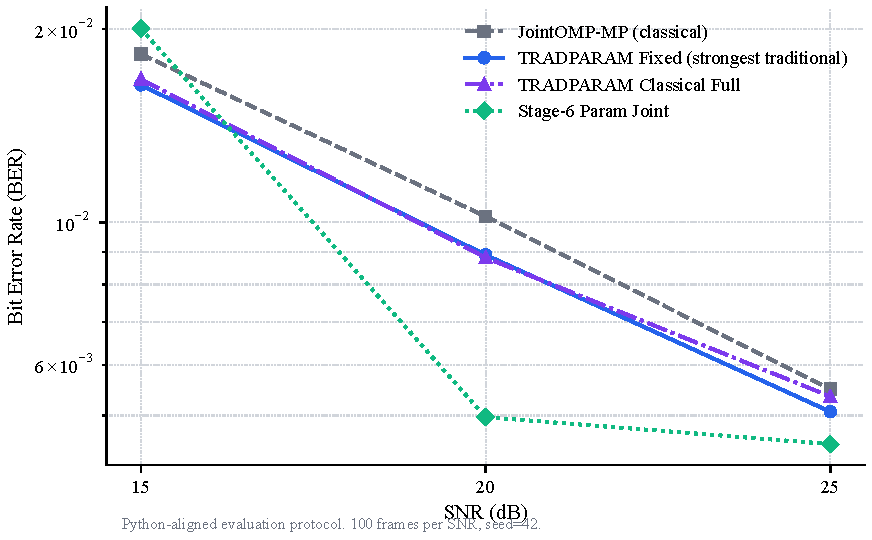
\includegraphics[width=0.72\textwidth]{figures/fyp_fig2_traditional_ber.pdf}
    \caption{BER vs.\ SNR for the traditional receiver family under the Python-aligned evaluation
             protocol. \texttt{TRADPARAM\,Fixed} is the strongest clean traditional representative,
             outperforming \texttt{JointOMP-MP} at verified SNR points.
             \texttt{CurrentJoint} is included for reference.}
    \label{fig:traditional_ber}
\end{figure}

% ─── Fig. 2b: BER vs SNR — CurrentJoint vs Frozen Corrector ─────────────────
% Data: nominal and failure_ppaths15 regimes, SNR=[5,10,15,20,25] dB.
%
\begin{figure*}[t]
    \centering
    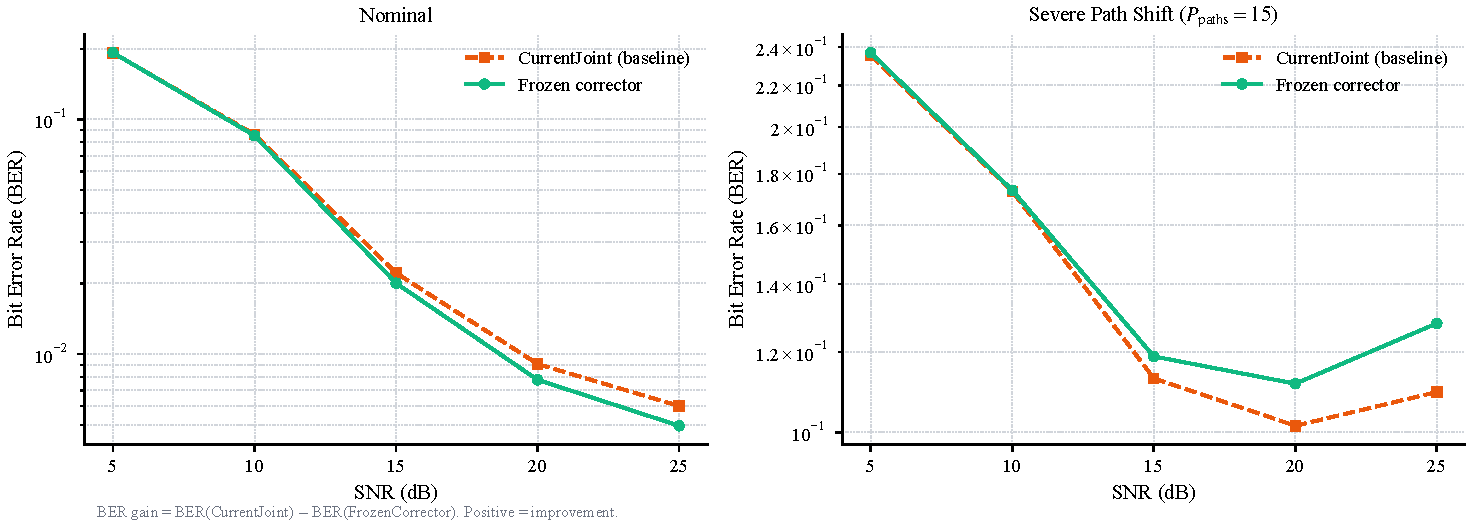
\includegraphics[width=0.96\textwidth]{figures/fyp_fig2b_corrector_ber_snr.pdf}
    \caption{BER vs.\ SNR for \texttt{CurrentJoint} baseline vs.\ frozen corrector
             in the nominal regime (\textit{left}) and the severe path-count shift $P_\text{paths}=15$
             (\textit{right}).
             Both panels use the corrected Python-aligned evaluation protocol on untouched test caches.
             In the nominal regime the corrector lies below the baseline curve;
             in the $P_\text{paths}=15$ regime it lies above, confirming the BER regression.
             BER gain = BER(CurrentJoint) $-$ BER(FrozenCorrector); positive means improvement.}
    \label{fig:corrector_ber_snr}
\end{figure*}

% ─── Fig. 3: Regime BER Gains + 95\% CI (forest plot) ───────────────────────
\begin{figure}[t]
    \centering
    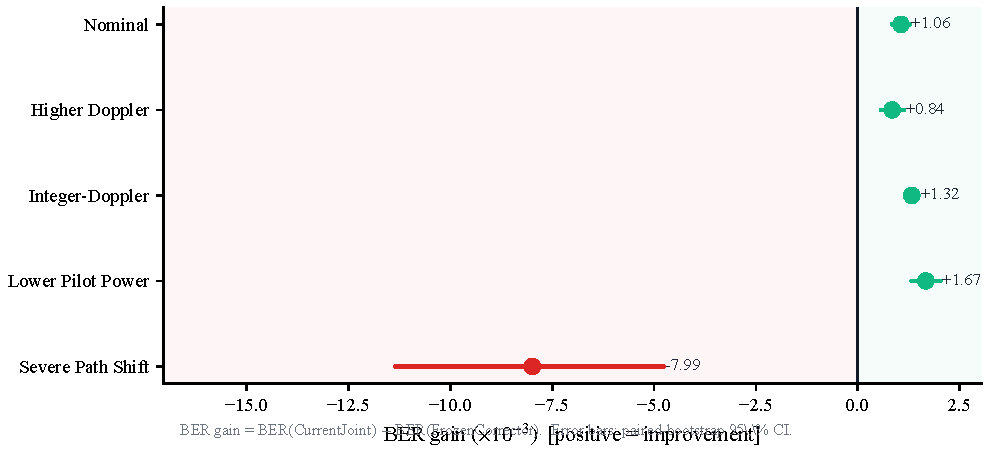
\includegraphics[width=0.72\textwidth]{figures/fyp_fig3_regime_gains.pdf}
    \caption{Mean BER gain of the frozen corrector across five evaluation regimes.
             Whiskers show paired-bootstrap 95\,\% CIs.
             BER gain = BER(CurrentJoint) $-$ BER(FrozenCorrector) on untouched test caches.
             Four regimes remain above zero; the severe path-count shift ($P_\text{paths}=15$)
             is cleanly negative, marking an explicit failure boundary.}
    \label{fig:regime_gains}
\end{figure}

% ─── Fig. 4: Feature-Group Ablation ─────────────────────────────────────────
\begin{figure}[t]
    \centering
    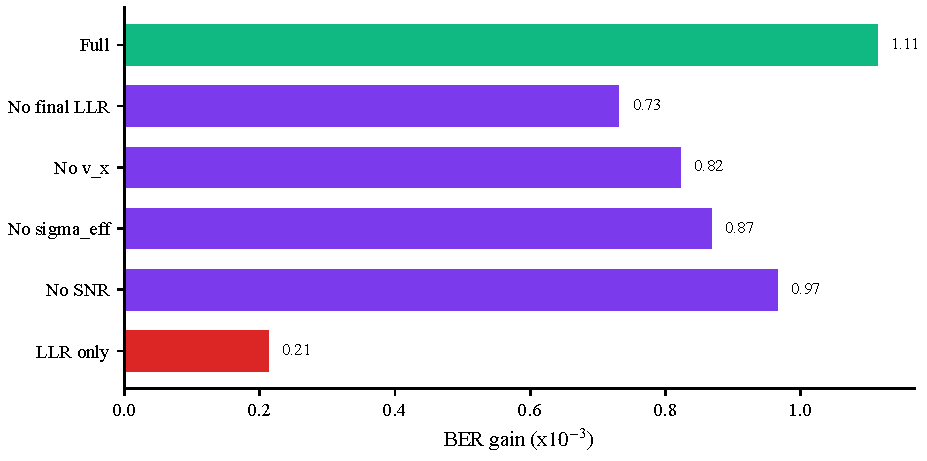
\includegraphics[width=0.72\textwidth]{figures/fig4_feature_ablation.pdf}
    \caption{Feature-group ablation of the frozen corrector on nominal untouched caches.
             The full 12-dimensional observable feature set achieves the highest BER gain.
             Restricting to LLR-only retains only $\approx19\,\%$ of the full gain,
             showing that the corrector is not merely an LLR threshold.}
    \label{fig:feature_ablation}
\end{figure}

% ─── Fig. 5: Packet-Level Utility ───────────────────────────────────────────
\begin{figure}[t]
    \centering
    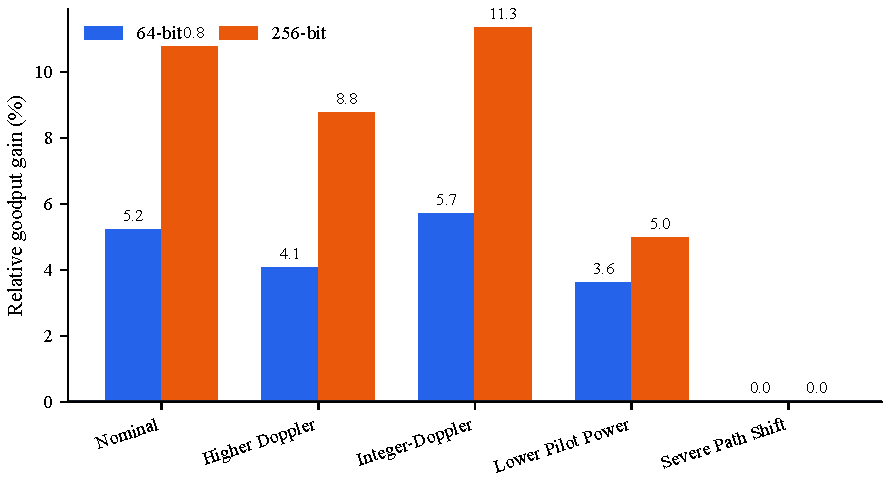
\includegraphics[width=0.72\textwidth]{figures/fig3_system_impact.pdf}
    \caption{Relative goodput gains for 64-bit and 256-bit contiguous packets under an
             uncoded ARQ-style proxy. Small BER gains amplify into meaningful endpoint
             improvements in the four positive regimes. The severe path-count shift
             ($P_\text{paths}=15$) yields no reliable gain at either packet length.}
    \label{fig:packet_utility}
\end{figure}

% ─── Fig. 6: Correction-Behavior Analysis ────────────────────────────────────
% Both panels now have real data from evaluate_frozen_direct_bit_corrector runs.
%
\begin{figure*}[t]
    \centering
    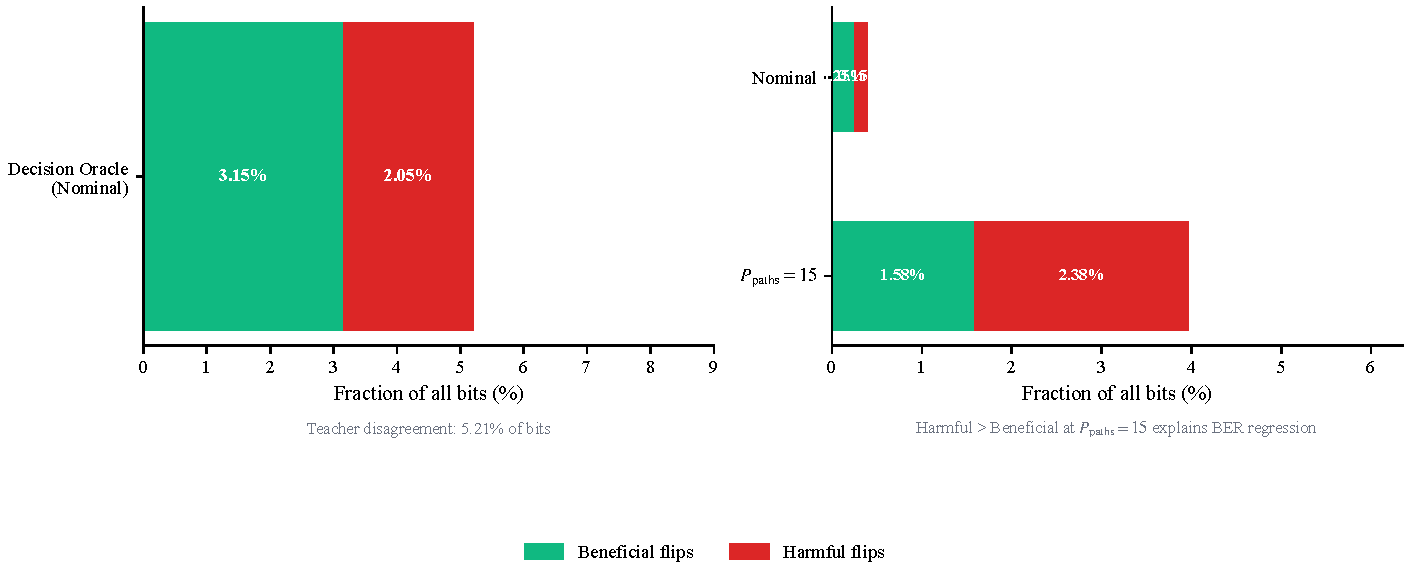
\includegraphics[width=0.96\textwidth]{figures/fyp_fig6_correction_behavior.pdf}
    \caption{Correction-behavior analysis.
             \textit{Left}: Decision-oracle headroom on the nominal held-out cache.
             Of all bits, $5.21\,\%$ are teacher-different; $3.15\,\%$ are oracle-beneficial flips
             and $2.05\,\%$ are oracle-harmful.
             \textit{Right}: Frozen corrector flip analysis (to be populated from experiment logs).
             The contrast between the nominal and $P_\text{paths}=15$ regimes is expected to show
             why the severe path-count shift causes BER regression.}
    \label{fig:correction_behavior}
\end{figure*}

% ─── Table 1: Traditional Receiver Family ────────────────────────────────────
% NOTE: BER values are \textit{---} until filled from experiment logs.
% TABLE1_traditional.tex — generated by gen_fyp_table1_traditional.py
\begin{table}[t]
\centering
\caption{Traditional receiver family comparison at SNR\,=\,15\,dB under the Python-aligned evaluation protocol (100 frames, seed\,=\,42). TRADPARAM Fixed is the strongest clean traditional representative, outperforming JointOMP-MP. CurrentJoint (learned backbone) is included for context.}
\label{tab:traditional_receivers}
\setlength{\tabcolsep}{5pt}
\begin{tabular}{lllll}
\toprule
\textbf{Method} & \textbf{Key Idea} & \textbf{Protocol} & \textbf{SNR (dB)} & \textbf{BER} \\
\midrule
JointOMP-MP & OMP one-shot support lock + iterative message-passin... & Python-aligned & 15 dB & 1.8291e-02 \\
TRADPARAM Fixed & Fixed traditional scaffold; sparse support + iterati... & Python-aligned & 15 dB & 1.6377e-02 \\
TRADPARAM Classical Full & Traditional scaffold with learnable classical scalar... & Python-aligned & 15 dB & 1.6709e-02 \\
CurrentJoint & Fully learned AFDM joint receiver backbone (deep unr... & Python-aligned & 15 dB & 2.2157e-02 \\
\bottomrule
\end{tabular}
\end{table}


% ─── Table 2: Method Comparison (FYP version) ────────────────────────────────
% TABLE2_fyp_method_comparison.tex — generated by gen_fyp_table2_method_comparison.py
\begin{table*}[t]
\centering
\caption{Method evolution under the corrected evaluation protocol. The ``Outcome after correction'' column shows what changed once the evaluation bug was fixed. The status column indicates the role each method plays in the final narrative.}
\label{tab:fyp_method_evolution}
\setlength{\tabcolsep}{4pt}
\begin{tabular}{p{2.4cm}p{2.0cm}p{2.4cm}p{3.6cm}p{3.0cm}}
\toprule
\textbf{Method} & \textbf{Family} & \textbf{Protocol} & \textbf{Outcome after correction} & \textbf{Status} \\
\midrule
JointOMPMP & Classical iterative & MATLAB direct eval & Superseded by Python-aligned protocol; TRADPARAM Fixed outperforms at verified SNR points & retained as historical reference \\
CurrentJoint & Learned (deep unrolled) & Python corrected & Retained as the base receiver for the final method & retained as backbone \\
vx\_recal\_v1 & Detector calibration & corrected same-test-set & Dropped after correction. No benefit over backbone. & \textit{Dropped} \\
distill\_pure\_iter0 & Mean-residual distillation & corrected same-test-set & Dropped. Decision audit showed headroom is sparse/boundary-local, not smooth mean-level. & \textit{Dropped} \\
Split-specific direct-bit corrector & Observable correction (probe) & split-specific probe & Viable but not generalised. Motivates frozen train-once design. & \textit{Bridge} \\
Frozen direct-bit corrector & Final method & train-once/test-on-many & Main contribution. Positive CI in 4 regimes; explicit failure at P\_paths=15. & \textbf{Main contribution} \\
\bottomrule
\end{tabular}
\end{table*}


% ─── Table 3: Scope / Claim Matrix (FYP version) ─────────────────────────────
% TABLE3_fyp_claim_scope.tex — generated by gen_fyp_table3_scope.py
\begin{table*}[t]
\centering
\caption{Scope and boundary matrix. Every claim is paired with its key evidence, the scope under which it holds, and the explicit boundary or limitation. Claims marked with a failure boundary are part of the reported result.}
\label{tab:fyp_claim_scope}
\setlength{\tabcolsep}{4pt}
\begin{tabular}{p{3.2cm}p{3.2cm}p{2.8cm}p{3.6cm}}
\toprule
\textbf{Claim} & \textbf{Key evidence} & \textbf{Scope} & \textbf{Explicit boundary} \\
\midrule
Mean-residual correction is not decision-effective under corrected evaluation & Corrected same-test-set comparison; CurrentJoint, vx\_recal\_v1, distill\_pure\_iter0 indistinguishable & Current AFDM joint receiver setting, Python-aligned protocol & Does not claim that residual correction always fails; specific to this receiver and setting \\
Frozen decision-level corrector yields reproducible BER gains & 3 untouched nominal caches; gain 1.059e-03, CI [8.42e-04, 1.27e-03]; std 5.53e-05 & Train-once/test-on-many; same AFDM simulator family; 10-25 dB SNR range & Reproducibility demonstrated for one trained instance; multi-seed training characterisation pending \\
Gain transfers across 3 regime shifts & Doppler 8.43e-04, integer-Doppler 1.32e-03, rho=0.4 1.67e-03; all bootstrap CIs above zero & Internal regime shifts within AFDM simulator family; same corrector weights, no retraining & Does not hold for P\_paths=15 (severe structural shift); not tested outside simulator family \\
Explicit failure boundary at P\_paths=15 & BER regression -7.99e-03; CI [-1.14e-02, -4.78e-03]; packet gain 0 & P\_paths=15 represents a harsh structural shift outside the training distribution & This IS the scope boundary — it is part of the reported result, not an exclusion \\
Small BER gains yield operationally meaningful packet-level improvement & 64-bit nominal +5.22\%, 256-bit nominal +10.76\%; consistent across 4 positive regimes & Uncoded contiguous ARQ-style packet proxy only; not a full coded communication-stack result & Proxy is simplified. Gains may not directly translate to a real coded link-layer system. \\
\bottomrule
\end{tabular}
\end{table*}


% ─── Table 4: Complexity / Overhead (FYP version) ────────────────────────────
% TABLE4_fyp_complexity.tex — updated for the learned-classical fusion rule.
\begin{table}[t]
\centering
\caption{Deployment-time complexity of the four-parameter learned-classical fusion rule compared to the earlier frozen 12-feature BCE corrector.  The classical teacher's compute cost is not tabulated here because it is already incurred by the classical receiver characterised in Section~\ref{ssec:midterm_uwa_results}; only the marginal cost of the fusion rule itself is shown.}
\label{tab:fyp_complexity}
\setlength{\tabcolsep}{5pt}
\begin{tabular}{lll}
\toprule
\textbf{Property} & \textbf{Fusion rule (this work)} & \textbf{BCE corrector (prior best)} \\
\midrule
Model type & Logistic regression & 2-hidden-layer MLP classifier \\
Input features & $[|\mu_\mathrm{teacher}|, |\mathrm{LLR}^\mathrm{model}|, \mathrm{SNR}]$ & $12$-D observable trajectory \\
Hidden layers & None & $2$ layers ($32, 16$ units) \\
Activation & Sigmoid output & ReLU hidden, sigmoid output \\
Total parameters & $\mathbf{4}$ & $961$ \\
Training data & Single training cache, $\approx 5.9 \times 10^{3}$ actionable bits & Single training cache, $\approx 10^{5}$ bits \\
Training time (commodity GPU) & $< 2$\,s & $\approx 30$\,s \\
Deployment & Frozen per-actionable-bit scalar rule & Frozen vectorised MLP pass per frame \\
Memory overhead & $16$\,B ($3 + 1$ float$32$) & $\approx 3.8$\,kB \\
Inference cost per actionable bit & $\approx 8$\,FLOPs & $\approx 1.8 \times 10^{3}$\,FLOPs \\
Marginal cost per $N = 512$ frame & $< 5 \times 10^{2}$\,FLOPs & $\approx 2.4 \times 10^{5}$\,FLOPs \\
\bottomrule
\end{tabular}
\end{table}

